\newpage
\section{Analisi del Problema}
\subsection{Analisi Documento dei Requisiti: Analisi delle Funzionalità}
\hfill \break

\textbf{Tabella delle Funzionalità}
\\

\begin{tabular} {|P{4cm}|P{4cm}|P{3.5cm}|P{4cm}|} % Qua cambiate a piacimento la larghezza
    \hline
    \textbf{Funzionalità} & \textbf{Tipo} & \textbf{Grado di complessità} & \textbf{Requisiti Collegati} \\
    \hline
    Gestione Farmacia & Memorizzazione dati e gestione dati & complessa & R5F, R9F, R10F, R11F, R12F, R13F, R14F, R15F \\
    \hline
    Registrazione & Interazione esterno e memorizzazione dati & semplice & R4F \\
    \hline
    RicercaFarmaci  &  Interazione esterno e lettura dati  &  semplice  &   R1F, R2F, R3F \\
    \hline
    Login  &  Interazione esterno e lettura dati  &  semplice  &   R7F \\
    \hline
    GestionePrenotazioni  &  Interazione esterno e memorizzazione dati  &  comp  &   R2F, R6F, R8F \\
    \hline
    ScritturaLog  &  Memorizzazione dati  &  semplice  &   R16F \\
    \hline
\end{tabular}
\\
\hfill \break

\textbf{GestioneFarmacia: Tabella Informazioni/Flusso}
\\

\begin{tabular} {|P{3cm}|P{3cm}|P{3cm}|P{3cm}|P{3cm}|}
    \hline
    \textbf{Informazione} & \textbf{Tipo} & \textbf{Livello protezione/privacy} & \textbf{Input / Output} & \textbf{Vincoli}\\
    \hline
    Nome Cliente & semplice & Protezione alta & Output & Non più di 40 caratteri \\
    \hline
    Cognome Cliente & semplice & Protezione alta & Output & Non più di 40 caratteri \\
    \hline
    Codice Fiscale Cliente & semplice & Protezione media & Output & Deve essere di 16 caratteri \\
    \hline
    Stato Cliente & semplice & Protezione media & Output & \\
    \hline
    Lista Farmaci & composto & Protezione alta & Output & \\
    \hline
    Lista Prenotazioni & composto & Protezione molto alta & Output & \\
    \hline
\end{tabular}
\hfill \break

\textbf{RicercaFarmaci: Tabella Informazioni/Flusso}
\\

\begin{tabular} {|P{3cm}|P{3cm}|P{3cm}|P{3cm}|P{3cm}|}
    \hline
    \textbf{Informazione} & \textbf{Tipo} & \textbf{Livello protezione/privacy} & \textbf{Input / Output} & \textbf{Vincoli}\\
    \hline
    Nome Farmaco & semplice & Protezione bassa & Input & \\
    \hline
    Località Utente & composto & Protezione alta & Input & \\
    \hline
    Farmacia & semplice & Protezione bassa & Input & \\
    \hline
    Lista Farmacie Pertinenti & composto & Protezione bassa & Output & Non più di 10 farmacie \\
    \hline
\end{tabular}
\hfill \break

\newpage
\textbf{Registrazione: Tabella Informazioni/Flusso}
\hfill \break

\begin{tabular} {|P{3cm}|P{3cm}|P{3cm}|P{3cm}|P{3cm}|}
    \hline
    \textbf{Informazione} & \textbf{Tipo} & \textbf{Livello protezione/privacy} & \textbf{Input/Output} & \textbf{Vincoli} \\
    \hline
    Nome Cliente & Semplice & Protezione media & Input & Non più di 40 caratteri \\
    \hline
    Cognome Cliente & semplice & Protezione media & Input & Non più di 40 caratteri \\
    \hline
    Data di Nascita & semplice & Protezione media & Input & Deve avere più di 16 anni e data di nascita successiva al 1900 \\
    \hline
    Codice Fiscale & semplice & Protezione media & Input & Deve essere di 16 caratteri \\
    \hline
    Email &  semplice & Protezione alta & Input & Deve essere di 256 caratteri e del formato giusto \\
    \hline
    Password & semplice & Protezione molto alta & Input & Deve essere almeno di 8 caratteri, di cui uno alfabetico e uno numerico \\
    \hline
\end{tabular}
\hfill \break

\textbf{ScritturaLog: Tabella Informazioni/Flusso}
\hfill \break

\begin{tabular} {|P{3cm}|P{3cm}|P{3cm}|P{3cm}|P{3cm}|}
    \hline
    \textbf{Informazione} & \textbf{Tipo} & \textbf{Livello protezione/privacy} &  \textbf{Input/Output} & \textbf{Vincoli} \\
    \hline
    Data  & semplice & Protezione media & Input & Non più di 40 caratteri \\
    \hline
    Ora & semplice & Protezione media & Input & Non più di 40 caratteri \\
    \hline
    Attore & semplice & Protezione alta & Input & Non più di 20 caratteri \\
    \hline
    Identificativo Farmacia & semplice & Protezione alta & Input & Non più di 20 caratteri \\
    \hline
    Operazione Eseguita & composto & Protezione alta & Input & \\
    \hline
    Evento & composto & Protezione molto alta & Input &  \\
    \hline
\end{tabular}
\hfill \break

\textbf{Login: Tabella Informazioni/Flusso}
\hfill \break

\begin{tabular} {|P{3cm}|P{3cm}|P{3cm}|P{3cm}|P{3cm}|}
    \hline
    \textbf{Informazione} & \textbf{Tipo} & \textbf{Livello protezione/privacy} & \textbf{Input/Output} & \textbf{Vincoli} \\
    \hline
    Email & semplice & Protezione molto alta & Input & Non più di 256 caratteri \\
    \hline
    Password & semplice & Protezione molto alta & Input & Non più di 50 caratteri \\
    \hline
\end{tabular}
\hfill \break

\textbf{GestionePrenotazione: Tabella Informazioni/Flusso}
\hfill \break

\begin{tabular} {|P{3cm}|P{3cm}|P{3cm}|P{3cm}|P{3cm}|}
    \hline
    \textbf{Informazione} & \textbf{Tipo} & \textbf{Livello protezione/privacy} & \textbf{Input/Output} & \textbf{Vincoli} \\
    \hline
    Data invio & semplice & Protezione media & Input & Non più di 40 caratteri \\
    \hline
    Ora invio & semplice & Protezione media & Input & Non più di 40 caratteri \\
    \hline
    Data prenotazione & semplice & Protezione media & Input & Solo una data compresa tra il giorno successivo e 14 giorni dopo \\
    \hline
    Elenco farmaci & composto & Protezione alta & Input & 1. Non più di 5 elementi per ogni farmaco <br> 2. Non più di 20 elementi in totale \\
    \hline
    Identificativo farmacia & semplice & Protezione alta & Input & Non più di 20 caratteri \\
    \hline
    Identificativo cliente & semplice & Protezione molto alta & Input & Non più di 20 caratteri \\
    \hline
    Lista prenotazioni  &  composto  &  Protezione alta  &  Output  &  \\
    \hline
\end{tabular}

\newpage
\subsubsection{Analisi Documento dei Requisiti: Analisi dei Vincoli}
\hfill \break

\textbf{Tabella Vincoli}
\hfill \break

\begin{tabular} {|P{3cm}|P{2.5cm}|P{3.5cm}|P{6cm}|}
    \hline
    \textbf{Requisito} & \textbf{Categorie} & \textbf{Impatto} & \textbf{Funzionalità} \\
    \hline
    Semplicità dell'interfaccia & Usabilità & Intuitività di utilizzo &  GestioneFarmacia, Registrazione, RicercaFarmaci, Login, NuovaPrenotazione  \\
    \hline
    Velocità della ricerca dei dati & Tempo di Risposta & Maggiore reattività & GestioneFarmacia, Registrazione, RicercaFarmaci, Login, NuovaPrenotazione \\
    \hline
    Velocità di memorizzazione dei dati & Tempo di Risposta & Maggiore reattività & GestioneFarmacia, Registrazione, Login, NuovaPrenotazione \\
    \hline
    Controllo Accessi &  Sicurezza  &  Peggiorano tempo di risposta e usabilità, migliorano la privacy dei dati  &  GestioneFarmacia, NuovaPrenotazione  \\
    \hline
    Protezione dei Dati &  Sicurezza  &  Peggiorano tempo di risposta, migliorano la privacy dei dati  &  GestioneFarmacia, Registrazione, RicercaFarmaci, Login, NuovaPrenotazione  \\
    \hline
\end{tabular}

\newpage

\subsubsection{Analisi Documento dei Requisiti: Analisi delle Interazioni}
\hfill \break

\textbf{Tabella Maschere}
\hfill \break

\begin{tabular} {|P{3.5cm}|P{7cm}|P{5cm}|}
    \hline
    \textbf{Maschera} & \textbf{Informazioni} & \textbf{Funzionalità} \\
    \hline
    Home Gestione & messaggio di benvenuto e scelta della funzionalità & GestioneFarmacia \\
    \hline
    View Login & email, password & Login \\
    \hline
    View Prenotazioni & lista prenotazioni & GestioneFarmacia \\
    \hline
    View ResocontoUtenti & nome cliente, cognome cliente, codice fiscale cliente, stato cliente & GestioneFarmacia \\
    \hline
    View VerificaIdentità & nome cliente, cognome cliente, codice fiscale cliente  & VeriticaIdentità \\
    \hline
    View Farmaci & lista farmaci & gestioneFarmacia \\
    \hline
    Home Servizio & messaggio di benvenuto, nome farmaco, località utente, lista farmacie pertinenti & RicercaFarmaci \\
    \hline
    View Registrazione &  nome cliente, cognome cliente, data di nascita, codice fiscale, email, password  & Registrazione \\
    \hline
    View NuovaPrenotazione & data invio, ora invio, data prenotazione, elenco farmaci, identificativo farmacia, identificativo cliente & NuovaPrenotazione \\
    \hline
    View PrenotazioniPersonali & lista prenotazioni & ListaPrenotazioni \\
    \hline
\end{tabular}
\hfill \break
\hfill \break

\textbf{Tabella Sistemi Esterni}
\hfill \break

\begin{tabular} {|P{3cm}|P{4cm}|P{4cm}|P{4cm}|}
    \hline
    \textbf{Sistema} & \textbf{Descrizione} & \textbf{Protocollo di Interazione} & \textbf{Livello di Sicurezza} \\
    \hline
    Gestione Magazzino  &  Sistema che si occupa della gestione dei farmaci in magazzino  &  GestioneMagazzino mette a disposizione delle funzionalità di elencazione dei farmaci  & Medio livello di sicurezza perchè protegge i dati della farmacia  \\
    \hline
\end{tabular}
\hfill \break

\newpage
\subsubsection{Analisi Ruoli e Responsabilità}
\hfill \break

\textbf{Tabella Ruoli}
\hfill \break

\begin{tabular} {|P{2.5cm}|P{3cm}|P{3.5cm}|P{3cm}|P{3cm}|}
    \hline
    \textbf{Ruolo} & \textbf{Responsabilità} & \textbf{Maschere} & \textbf{Riservatezza} & \textbf{Numerosità} \\
    \hline
    Farmacista & Gestione di tutte le informazioni relative agli utenti e alle prenotazioni di una farmacia & Home Gestione, View Login, View Prenotazioni, View ResocontoUtenti, View VerificaIdentità, View Farmaci,  & È richiesto un alto grado di riservatezza  & Massimo 10 farmacisti per ogni farmacia \\
    \hline
    Cliente & Ricerca di un farmaco senza necessità di login & Home Servizio, View Login, View Registrazione  & È richiesto un medio grado di riservatezza & Illimitati \\
    \hline
    % roba molto brutta ma non so perchè non va a capo automaticamente questo
    ClienteRegi- strato & Ricerca e prenotazione di farmaci presso una farmacia & Home Servizio, View NuovaPrenotazione, View PrenotazioniPersonali &  È richiesto un alto grado di riservatezza  & Illimitati \\
    \hline
\end{tabular}
\hfill \break
\hfill \break

\textbf{Farmacista: Tabella Ruolo-Informazioni}
\hfill \break

\begin{tabular} {|P{7cm}|P{7cm}|}
    \hline
    \textbf{Informazione} & \textbf{Tipo di Accesso} \\
    \hline
    Nome Cliente & Lettura \\
    \hline
    Cognome Cliente & Lettura \\
    \hline
    Codice Fiscale & Lettura \\
    \hline
    Stato Cliente & Lettura/Scrittura \\
    \hline
    Lista Farmaci & Lettura/Scrittura \\
    \hline
    Lista Prenotazioni & Lettura/Scrittura \\
    \hline
\end{tabular}
\hfill \break
\hfill \break

\textbf{ClienteRegistrato: Tabella Ruolo-Informazioni}
\hfill \break

\begin{tabular} {|P{7cm}|P{7cm}|}
    \hline
    \textbf{Informazione} & \textbf{Tipo di Accesso} \\
    \hline
    Nome Cliente & Lettura/Scrittura \\ 
    \hline
    Cognome Cliente & Lettura/Scrittura \\
    \hline
    Data di Nascita & Lettura \\
    \hline
    Codice Fiscale & Lettura \\
    \hline
    Email & Lettura/Scrittura \\
    \hline
    Password & Lettura/Scrittura \\
    \hline
    Nome Farmaco & Scrittura \\
    \hline
    Località Utente & Lettura \\
    \hline
    Lista Farmacie Pertinenti  & Lettura \\
    \hline
    Data prenotazione & Scrittura \\
    \hline
    Elenco farmaci & Scrittura \\
    \hline
\end{tabular}

\textbf{Cliente: Tabella Ruolo-Informazioni}
\hfill \break

\begin{tabular} {|P{7cm}|P{7cm}|}
    \hline
    \textbf{Informazione} & \textbf{Tipo di Accesso} \\
    \hline
    Nome Farmaco & Scrittura \\
    \hline
    Località Utente & Scrittura \\
    \hline
    Lista Farmacie Pertinenti  & Lettura \\
    \hline
\end{tabular}
\hfill \break
\hfill \break

\subsubsection{Scomposizione del Problema}
\hfill \break

\textbf{Tabella Scomposizione Funzionalità}
\hfill \break

\begin{tabular} {|P{7cm}|P{7cm}|}
    \hline
    \textbf{Funzionalità} & \textbf{Scomposizione} \\
    \hline
    GestioneFarmacia &  ResocontoFarmaci, ResocontoUtenti, ControlloPrenotazioni, VerificaIdentità  \\
    \hline
    GestionePrenotazioni  &  NuovaPrenotazione, ListaPrenotazioni  \\
    \hline
    ControlloPrenotazioni  &  ConfermaPrenotazione  \\
    \hline
    ResocontoUtenti &  SospensioneUtenza  \\
    \hline
\end{tabular}
\\

\break
Non sono presenti legami di esclusione o di necessità tra le sotto-funzionalità del sistema. 
\hfill \break

\newpage
\subsubsection{Creazione Modello del Dominio}

Il seguente diagramma delle classi rappresenta la parte di modello del dominio relativa al sistema. \\

\begin{figure}[h!]
    \begin{center}
        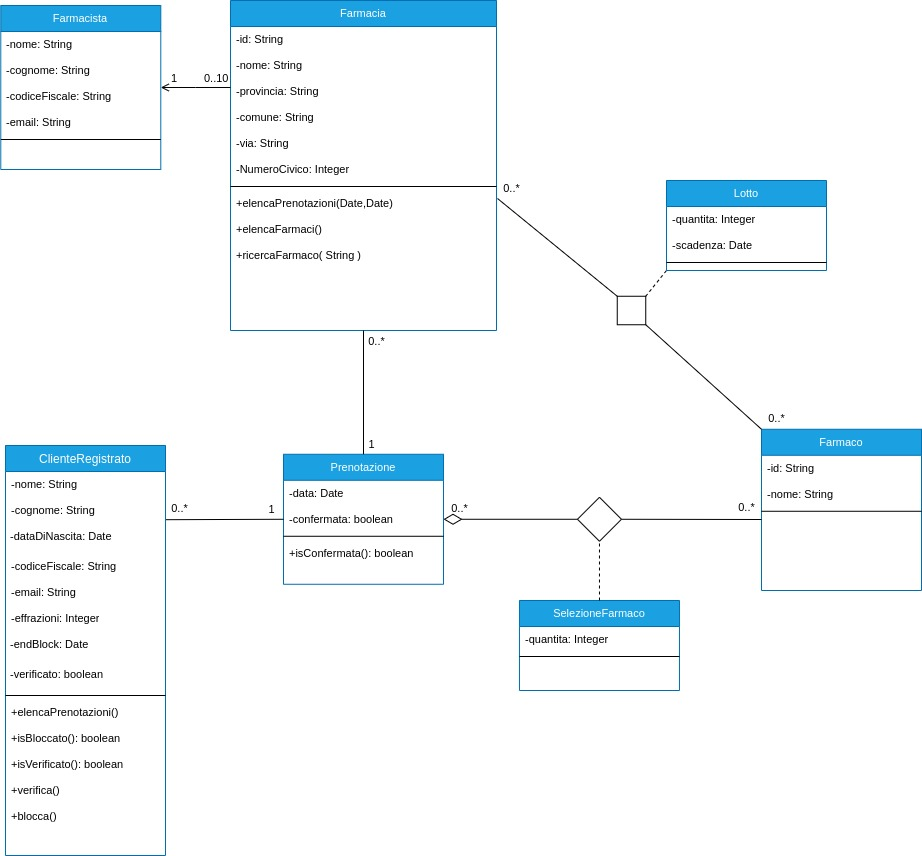
\includegraphics[width=\textwidth]{ModelloDominio.jpg}
    \end{center}
\end{figure}
\hfill \break

\newpage
\subsubsection{Architettura Logica: Struttura}
\hfill \break

\textbf{Diagramma dei package}
\hfill \break

\begin{figure}[h!]
    \begin{center}
        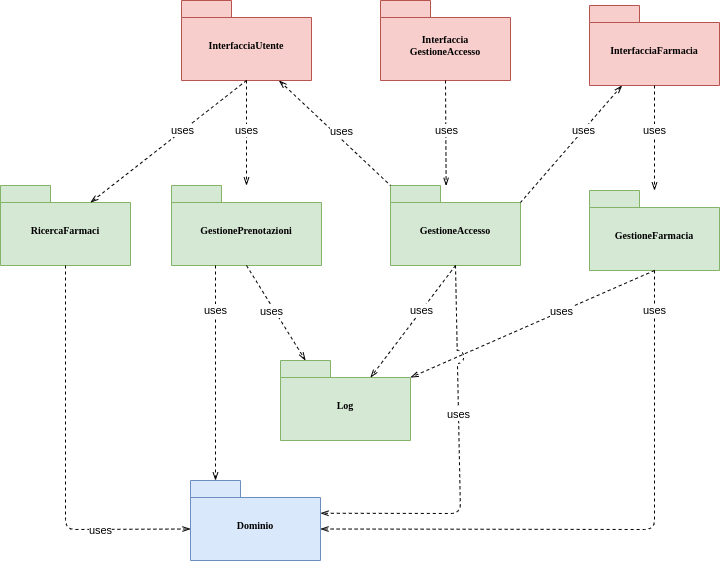
\includegraphics[scale=0.6]{Diagrammi-Package.png}
    \end{center}
\end{figure}
\hfill \break

\textbf{Diagramma delle classi: InterfacciaGestioneAccesso \& GestioneAccesso}
\hfill \break

\begin{figure}[h!]
    \begin{center}
        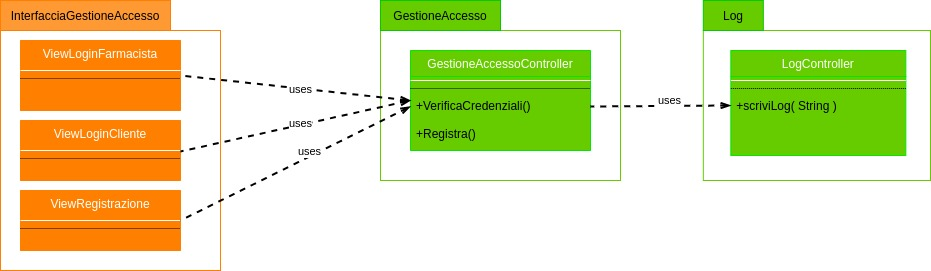
\includegraphics[width=\textwidth]{Diagrammi-Gestione Accesso.jpg}
    \end{center}
\end{figure}
\hfill \break

\textbf{Diagramma delle classi: InterfacciaGestioneFarmacia \& GestioneFarmacia}
\hfill \break

\begin{figure}[h!]
    \begin{center}
        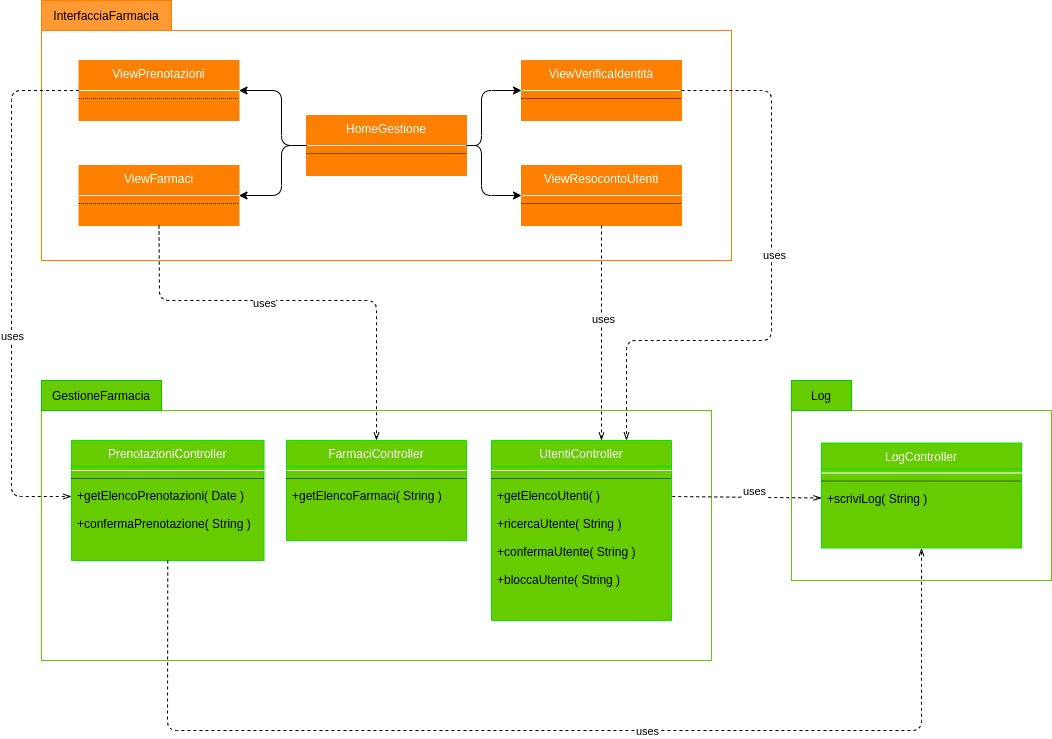
\includegraphics[width=\textwidth]{Diagrammi-Farmacia.jpg}
    \end{center}
\end{figure}
\hfill \break

\newpage
\textbf{Diagramma delle classi: InterfacciaUtente \& RicercaFarmaci \& GestionePrenotazioni }

\begin{figure}[h!]
    \begin{center}
        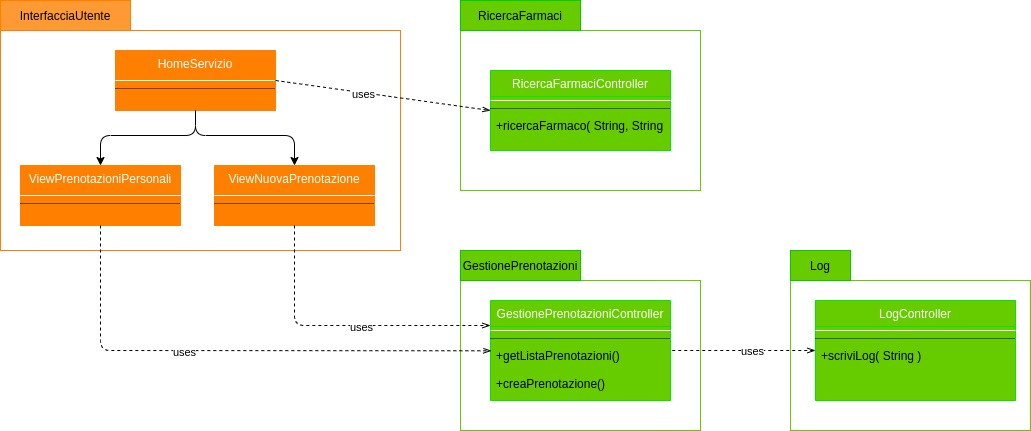
\includegraphics[width=\textwidth]{Diagrammi-Utente.jpg}
    \end{center}
\end{figure}
\hfill \break

\newpage
\subsubsection{Architettura Logica: Interazione}
\hfill \break

\textbf{Diagramma di Sequenza: Login Utente}

\begin{figure}[h!]
    \begin{center}
        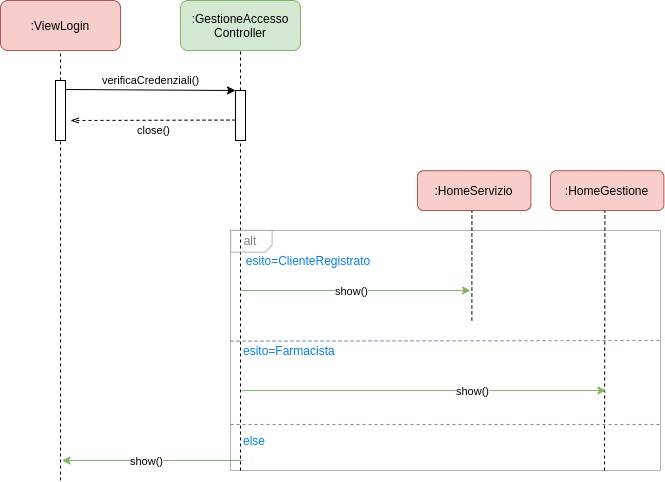
\includegraphics[scale=0.5]{Interazione-LoginUtente.jpg}
    \end{center}
\end{figure}
\hfill \break

\textbf{Diagramma di Sequenza: Registrazione Utente}

\begin{figure}[h!]
    \begin{center}
        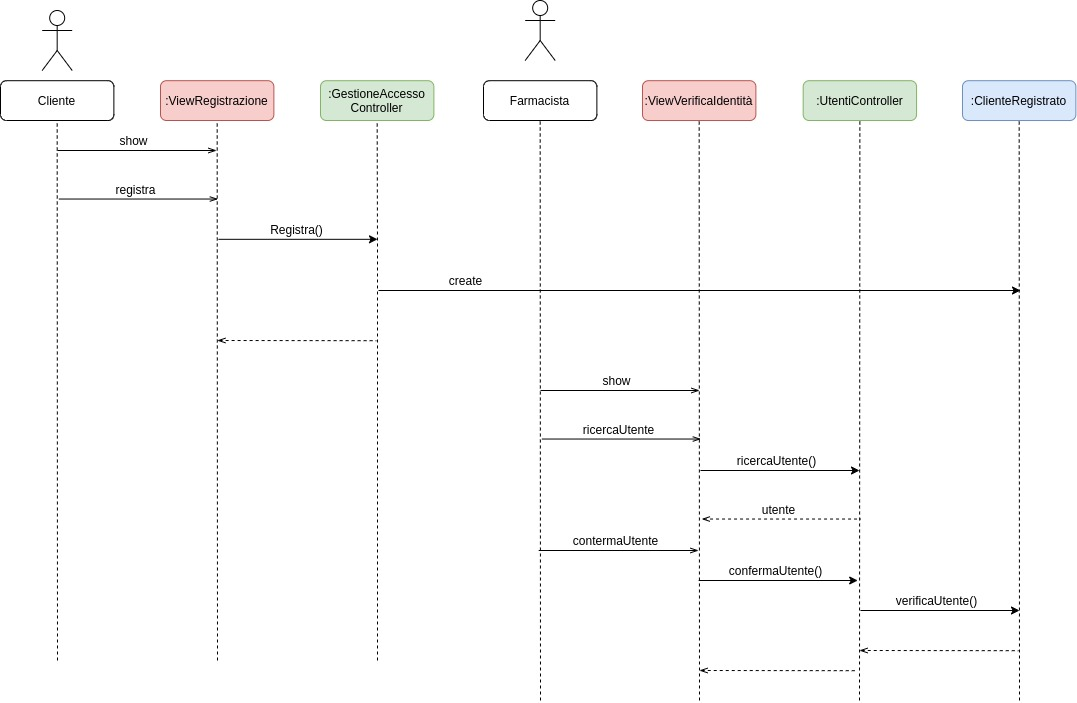
\includegraphics[scale=0.4]{Interazione-RegistrazioneUtente.jpg}
    \end{center}
\end{figure}
\hfill \break

\textbf{Diagramma di Sequenza: Nuova Prenotazione}

\begin{figure}[h!]
    \begin{center}
        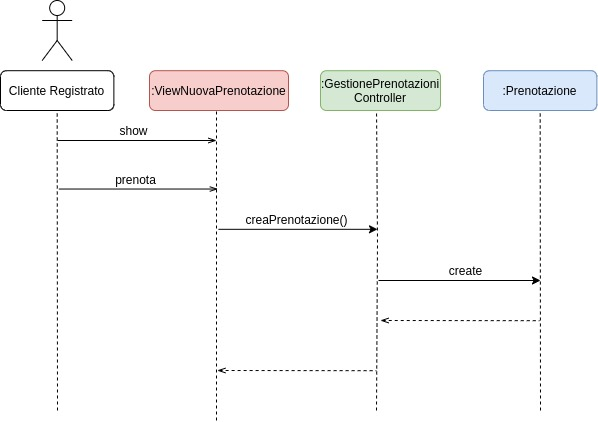
\includegraphics[scale=0.5]{Interazione-NuovaPrenotazione.jpg}
    \end{center}
\end{figure}
\hfill \break

\textbf{Diagramma di Sequenza: Conferma Prenotazione}

\begin{figure}[h!]
    \begin{center}
        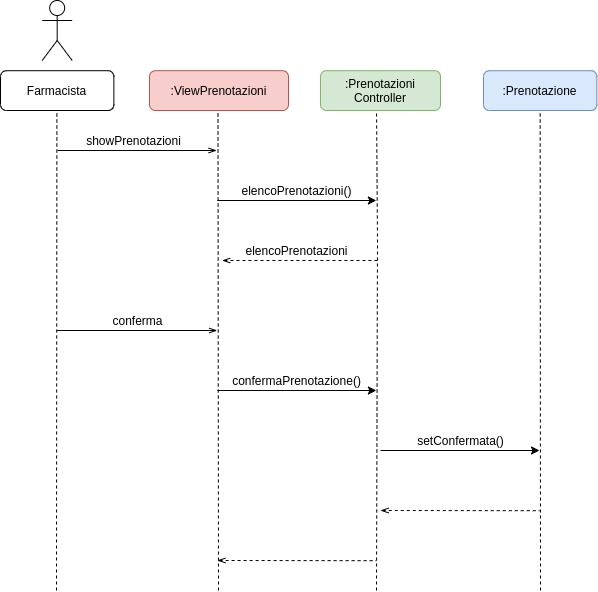
\includegraphics[scale=0.5]{Interazione-ConfermaPrenotazione.jpg}
    \end{center}
\end{figure}
\hfill \break

\textbf{Diagramma di Sequenza: Ricerca Farmaco}

\begin{figure}[h!]
    \begin{center}
        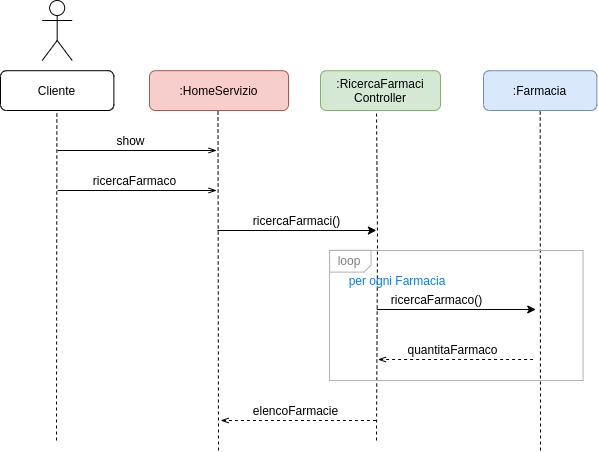
\includegraphics[scale=0.5]{Interazione-RicercaFarmaco.jpg}
    \end{center}
\end{figure}
\hfill \break

\textbf{Diagramma di Sequenza: Sospensione Utenza}

\begin{figure}[h!]
    \begin{center}
        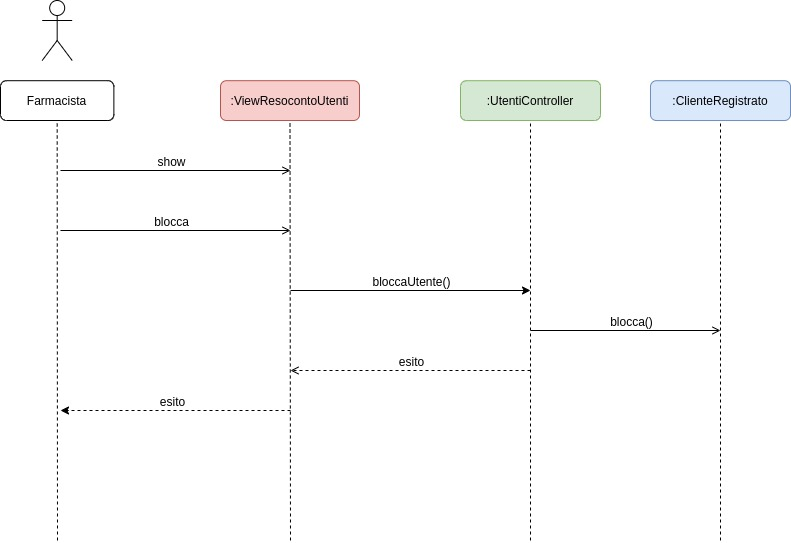
\includegraphics[scale=0.5]{Interazione-SospensioneUtenza.jpg}
    \end{center}
\end{figure}
\hfill \break

\newpage
\subsubsection{Architettura Logica: Comportamento}
\hfill \break

\textbf{Diagramma di Stato: Analizza Utente}

\begin{figure}[h!]
    \begin{center}
        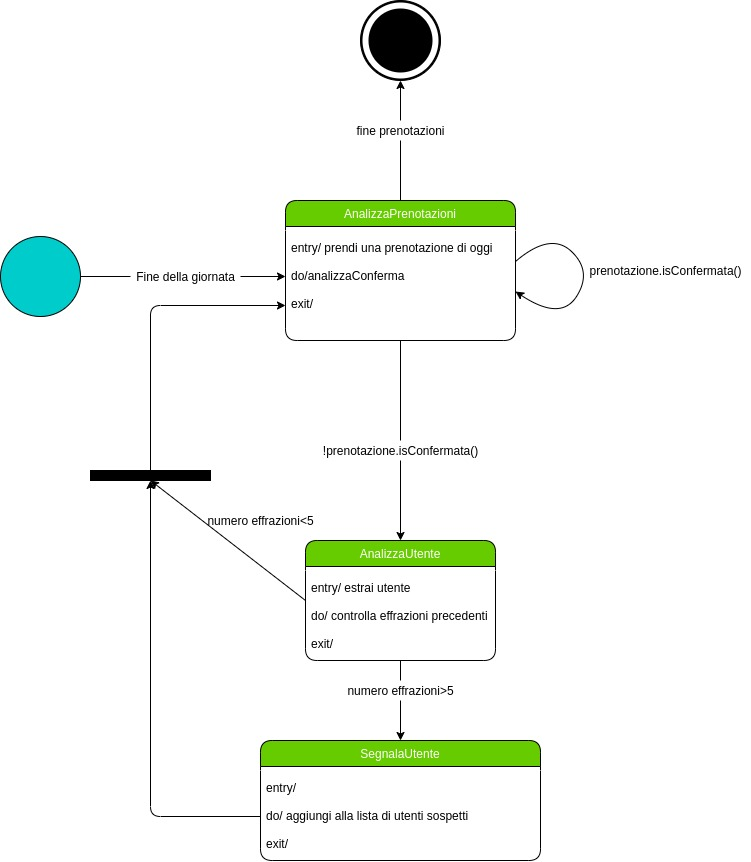
\includegraphics[scale=0.5]{Comportamento.jpg}
    \end{center}
\end{figure}
\hfill \break

\newpage
\subsubsection{Piano di Lavoro}

I compiti sono stati divisi in base alle competenze di 
ogni membro del gruppo come indicato nella tabella sottostante:\\

\begin{tabular} {|P{5cm}|P{5cm}|P{5cm}|} % Qua cambiate a piacimento la larghezza
    \hline
    \textbf{Package} & \textbf{Progetto} & \textbf{Sviluppo} \\
    \hline
    Dominio  &  Guerra,Palaferri,Romanini  &  Guerra\\
    \hline
    Log  &  Guerra,Palaferri,Romanini & Guerra\\
    \hline
    RicercaFarmaci  &  Guerra,Palaferri,Romanini &  Palaferri \\
    \hline
    GestionePrenotazioni  & Guerra,Palaferri,Romanini & Palaferri,Romanini \\
    \hline
    GestioneAccesso  & Guerra,Palaferri,Romanini & Guerra,Romanini \\
    \hline
    GestioneFarmacia  & Guerra,Palaferri,Romanini & Palaferri,Romanini \\
    \hline
    InterfacciaUtente  & Guerra,Palaferri,Romanini & Romanini \\
    \hline
    InterfacciaGestioneAccsso  & Guerra,Palaferri,Romanini & Guerra\\
    \hline
    InterfacciaFarmacia  & Guerra,Palaferri,Romanini & Palaferri,Romanini \\
    \hline
\end{tabular}
\hfill \break

I tempi di rilascio sono i seguenti:
\begin{itemize}
    \item Progettazione entro due settimane dalla data odierna
    \item Sviluppo dei vai moduli con annessi test unitari entro una settimana dalla fine della fase di progettazione
    \item Integrazione e testing del sistema entro una settimane dalla fine dello sviluppo
\end{itemize}
\hfill \break

\textbf{Sviluppi Futuri}
\\

Il cliente ha richiesto la creazione di un applicativo mobile per sistemi
android e iOS, con l'obbiettivo di rendere il più pratico possibile l'utilizzo
del programma.

\newpage
\subsubsection{Piano del Collaudo}

\usemintedstyle{manni}
\begin{minted}
[
frame=lines,
framesep=2mm,
baselinestretch=1.2,
bgcolor=LightGray,
fontsize=\footnotesize,
linenos
]
{java}
public class testPrenotazione{
    private Prenotazione prenotazione;

    @Before
    public void setUp(){
       prenotazione = new Prenotazione();
    }

    @Test
    public void testCostruttore(){
        prenotazione = new Prenotazione(new SimpleDateFormat("2021-06-01"), true);
        Assert.assertNull(prenotazione.isConfermata());
    }

    @Test
    public void testGetter(){
        prenotazione = new Prenotazione(new SimpleDateFormat("2021-06-01"), true);
        Assert.assertEquals(prenotazione.getData(), new SimpleDateFormat("2021-06-01"));
        Assert.assertEquals(prenotazione.getConfermata(), true);
    }

    @Test
    public void testSetter(){
        prenotazione.setData(new SimpleDateFormat("2021-07-02"));
        Assert.assertEquals(prenotazione.getData(), new SimpleDateFormat("2021-07-02"));
        prenotazione.setConfermata(true);
        Assert.assertEquals(prenotazione.getConfermata(), true);
    }
}

public class testFarmacia{
    private Farmacia farmacia;

    @Before 
    public void setUp(){
        farmacia = new Farmacia();
    }

    @Test
    public void testCostruttore(){
        Assert.assertNull(farmacia.getNome());
        Assert.assertNull(farmacia.getId());
    }

    @Test 
    public void testGetter(){
        farmacia = new Farmacia("N23N230SD", "Ubertini", "BO", "Bologna", "via Libia", "10");
        Assert.assertEquals(farmacia.getId(),"N23N230SD");
        Assert.assertEquals(farmacia.getNome(),"Ubertini");
        Assert.assertEquals(farmacia.getProvincia(),"BO");
        Assert.assertEquals(farmacia.getComune(),"Bologna");
        Assert.assertEquals(farmacia.getVia(),"via Libia");
        Assert.assertEquals(farmacia.getNumeroCivico(),"10");
    }

    @Test 
    public void testSetter(){
        farmacia.setId("N23N230SD");
        Assert.assertEquals(farmacia.getId(),"N23N230SD");
        farmacia.setNome("Ubertini");
        Assert.assertEquals(farmacia.getNome(),"Ubertini");
        farmacia.setProvincia("BO");
        Assert.assertEquals(farmacia.getProvincia(),"BO");
        farmacia.setComune("Bologna");
        Assert.assertEquals(farmacia.getComune(),"Bologna");
        farmacia.setVia("via Libia");
        Assert.assertEquals(farmacia.getVia(),"via Libia");
        farmacia.setNumeroCivico("10");
        Assert.assertEquals(farmacia.getNumeroCivico(),"10");
    }
}

public class testCliente{
    private ClienteRegistrato cliente;

    @Before 
    public void setUp(){
        cliente = new ClienteRegistrato();
    }

    @Test 
    public void testGetter(){
        cliente = new ClienteRegistrato("Federico", "Chesani", new
        SimpleDateFormat("1920-07-10"), "CHSFRC20L10A944G",
        "federico.chesani@unibo.it", 0, null, true, false);
        Assert.assertEquals(cliente.getNome(), "Federico");
        Assert.assertEquals(cliente.getCognome(), "Chesani");
        Assert.assertEquals(cliente.getNascita(), new SimpleDateFormat("1920-07-10"));
        Assert.assertEquals(cliente.getCodiceFiscale(), "CHSFRC20L10A944G");
        Assert.assertEquals(cliente.getEmail(), "federico.chesani@unibo.it");
        Assert.assertEquals(cliente.getEffrazioni(), 0);
        Assert.assertEquals(cliente.isVerificato(), true);
        Assert.assertEquals(cliente.isBloccato(), false);
    }

    @Test 
    public void testSetter(){
        cliente.setNome("Federico");
        Assert.assertEquals(cliente.getNome(), "Federico");
        cliente.setCognome("Chesani");
        Assert.assertEquals(cliente.getCognome(), "Chesani");
        cliente.setNascita(new SimpleDateFormat("1920-07-10"));
        Assert.assertEquals(cliente.getNascita(), new SimpleDateFormat("1920-07-10"));
        cliente.setCodiceFiscale("CHSFRC20L10A944G");
        Assert.assertEquals(cliente.getCodiceFiscale(), "CHSFRC20L10A944G");
        cliente.setEmail("federico.chesani@unibo.it");
        Assert.assertEquals(cliente.getEmail(), "federico.chesani@unibo.it");
        cliente.setEffrazioni(0);
        Assert.assertEquals(cliente.getEffrazioni(), 0);
        cliente.setVerificato(true);
        Assert.assertEquals(cliente.isVerificato(), true);
        cliente.setBloccato(false);
        Assert.assertEquals(cliente.isBloccato(), false);
    }
}
\end{minted}
